\chapter{Methodology}
\label{chap:2}
\ChapterPageStuff{2}

\section{Preamble}
In this chapter the methodology to create and implement a logging mechanism to do system utilisation analysis on software system will be discussed. In \Cref{sec:EventLogging} provided the needed literature to create a logging mechanism in \Cref{sec:Ch3_LoggingMechanism} for two software systems.

\section{Logging mechanism}\label{sec:Ch3_LoggingMechanism}
For this study two software systems are used to implement two different logging mechanisms. The first software system which will be called System A, is energy management system that uses \emph{PHP}. System B is a \emph{.NET Framework}\footnote{\label{ftn:NetFramework}\textbf{.NET Framework} is a run-time execution environment that consists of common language run-time (\emph{CLR}) and a \emph{.NET Framework Class Library} \cite{Harkness2007}.} system with a \emph{MVC} architecture as in \Cref{fig:ch2_Flow_MVC_Architecture} and is the administrative software system to configure System A.

\subsection{Logging points}
Logging point are essential data that describes the event's key features when creating a log as discussed in \Cref{sec:Ch1_LoggignPoints}. Both System A and B have certain key logging points that needs to be obtained from the user generated event.

\subsubsection{System A's logging points}
In \Cref{fig:ch2_SystemA_Dashboard} each mine group have multiple toolboxes linked to them. They can be same toolbox linked to both mine groups such as \emph{T1} and \emph{T3}. These toolboxes represent a group of dashboards related to the aspects of energy management of mines. Each of these toolboxes have a dashboards linked to them and each mine group can have different dashboards linked to the to the same toolbox. Each one of these mine groups, toolboxes and dashboards forms part of System A's web pages which the user can access where event logs are generated.

\begin{figure}[!htb] % An h :here, t: top, b: bottom.
	\centering % cent the figure
	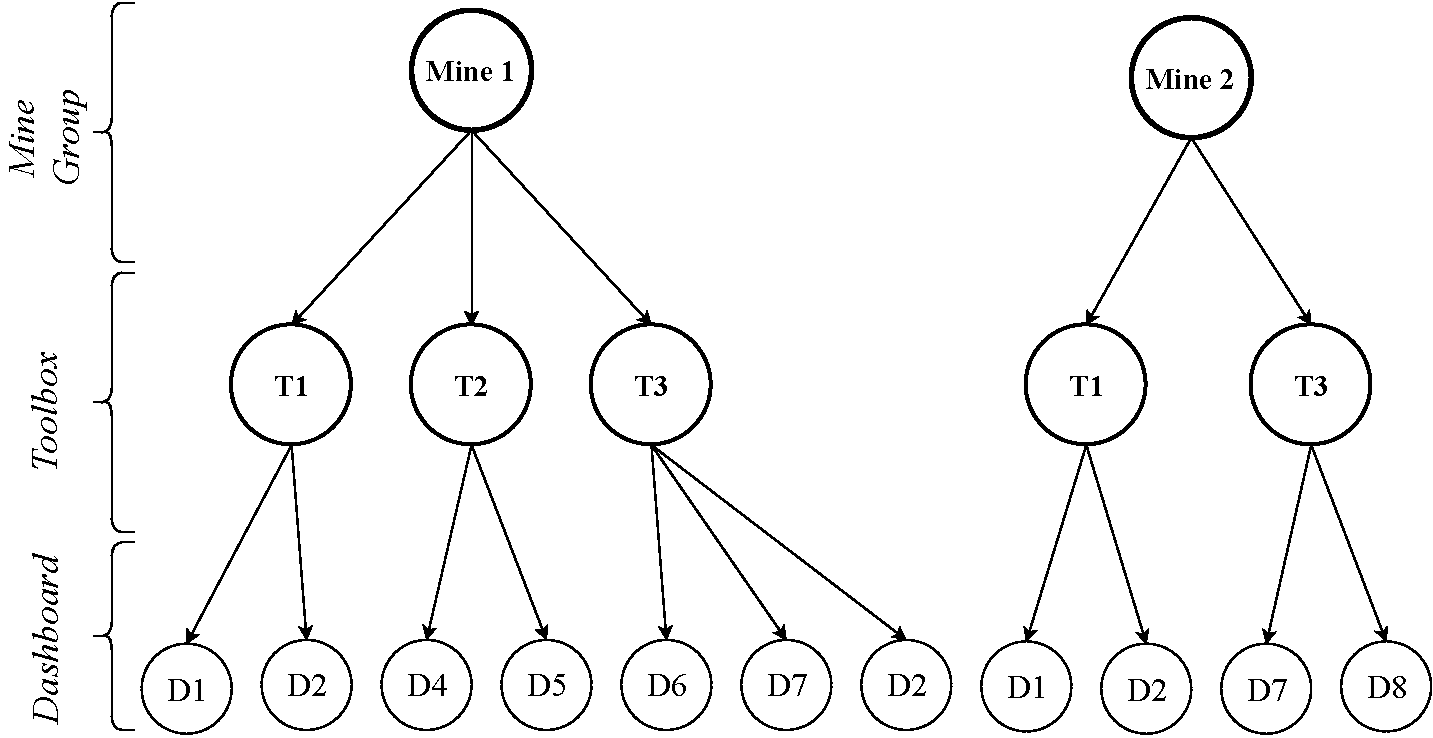
\includegraphics[width=0.9\textwidth]{Images/Chapter2/SystemA_Dashboard/SystemA_Dashboard.pdf}
	\caption[System A dashboard links]
	{\textit{System A dashboard links}}\label{fig:ch2_SystemA_Dashboard}
\end{figure}

The PHP session helps to keep to track of any information needed for these pages to be fully functional like the user's identity and dashboard related data. This information can be used to give insight on which page the user is currently active on. In this case for System A the important PHP session information is:

\begin{itemize}
	\item \textbf{User's identity:} The session contains the user's name and identity number which is the unique primary key for the user. This session information will always be available if the user is active on the software system from the instance they are logged in and verified until the user logs out and close their browser.
	\item \textbf{Group identity:} System A is used for multiple mine companies, each of the mining companies have a unique identity number. Each group have multiple toolboxes linked to them for energy management.
	\item \textbf{Dashboard identity:} Each dashboard uses the PHP files to construct a web page the user can view. To correctly navigate and get the correct page when the user request it, a unique identity number is used. In some cases for this system the same PHP file can be used for multiple dashboards as extra configuration data is obtained from the database for that specific dashboard identity number.
	\item \textbf{Configuration meta data identity:} In \Cref{fig:ch2_SystemA_Dashboard} the same dashboard can be linked to different mine groups or toolboxes. The PHP session contains any other identification parameters of which meta data should be loaded to configure the dashboard for the correct mine group and toolbox.
\end{itemize}

This key information is essential to define which key logging points the logging mechanism needs to get from the PHP session. In \Cref{tbl:Ch2_System_A_Logging_Points} System A's key logging points which are saved in a SQL database. Each logging point can be accessed either by the PHP session or other runtime data present when the event took place such as any meta data that as send back the server as request parameters.

\begin{table}[!htb]
	\centering
	\small
	\caption[Logging points]
	{\textit{System A user activities table}}
	\label{tbl:Ch2_System_A_Logging_Points}
	\begin{tabularx}{\textwidth}{|l|l|X|}
		\hline \textbf{Column Name} & \textbf{SQL Data Type} & \textbf{Description} \\
		\hline \textbf{ActivityID} & INT(11) & The activity identification is an incremental number of the event that is logged.\\
		\hline \textbf{Timestamp} & DATETIME & Foreign reference key to the Dashboard table.\\
		\hline \textbf{UserID} & INT(45) & Each user has a unique identifier which is a numerical identification number that is foreign key reference to the \emph{User} table.\\
		\hline \textbf{GroupID} & INT(4) & This foreign key reference to the Group table is contract groups identification number. \\ 		
		\hline \textbf{ActivityType} & ENUM & Each event that user initiated has an activity type as in \Cref{tbl:Ch2_SystemA_EventTypes}. \\
		\hline \textbf{File} & VARCHAR(200) & This the PHP file from which the request is processed.\\
		\hline \textbf{RequestParameters} & JSON & Request parameters of the event. This can also be other meta data is important to get that adds more information about the user's activity using certain controls on a dashboard or toolbox. \\
		\hline
	\end{tabularx}
\end{table}

\clearpage

The user activity types in \Cref{tbl:Ch2_SystemA_EventTypes} is the all the possible activities the user can generate in System A. The \emph{DetailView} activities is expected to the largest portion of events that will be tracked as users will generally try to use multiple input elements on the dashboard or toolbox. \par The \emph{Dash} event type is only useful to track which dashboards and toolboxes the user navigates to and it will not be accurate indicator to how much a dashboard or toolbox is used. The \emph{DetailView} and \emph{Report} user activity types is better representation of the utilisation of these software components as these events are the user's objectives using the software systems and not trying access the software systems.  

\begin{table}[!htb]
	\centering
	\small
	\caption[System A user activity types]
	{\textit{System A user activity types}}
	\label{tbl:Ch2_SystemA_EventTypes}
	\begin{tabularx}{\textwidth}{|l|X|}
		\hline \textbf{Activity Type} & \textbf{Description} \\
		\hline \textbf{Dash} & Any activity that the user attempts to access a toolbox or dashboard on System A is \emph{Dash} event type. \\
		\hline \textbf{DetailView} & Any other activities such as viewing certain dates data or editing and saving activities on System A is \emph{DetailView} events and have other meta data which is the request parameters send back to server. These events exclude \emph{Report} events. \\
		\hline \textbf{Report} & There are multiple detailed reports generated on these dashboards which are classified as \emph{Report} events. \\
		\hline
	\end{tabularx}
\end{table}

Using the key logging points of \Cref{tbl:Ch2_System_A_Logging_Points} the \emph{ERD} for all the tables used to for System A user activity logging data is created in \Cref{fig:Ch2_SystemA_Basic_ERD}. Table \emph{SystemA\_UserActvities} is where all the user activity tracking data is stored with foreign key references to the \emph{Dashboards}, \emph{Users} and \emph{Group} tables.

\begin{figure}[!htb] % An h :here, t: top, b: bottom.
	\centering % cent the figure
	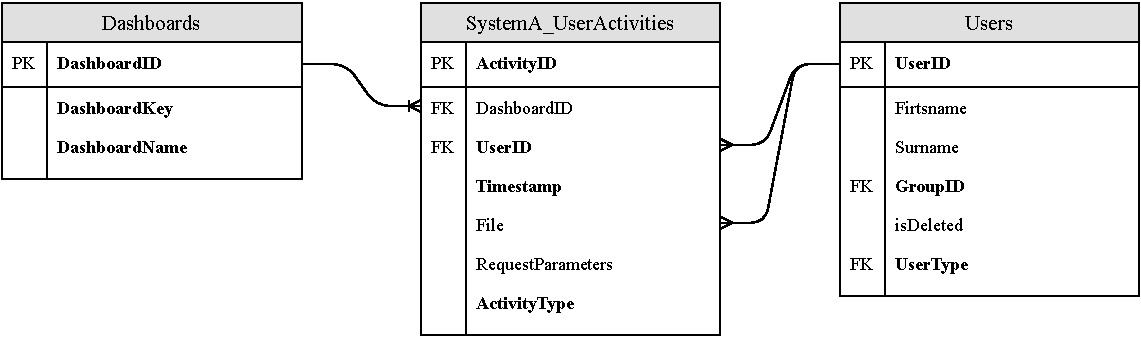
\includegraphics[width=0.95\textwidth]{Images/Chapter2/SystemA_ERD_Basic/SystemA_ERD_Basic.pdf}
	\caption[System A user activity ERD]
	{\textit{System A user activity ERD}}\label{fig:Ch2_SystemA_Basic_ERD}
\end{figure}

\clearpage

\subsubsection{System B's logging points}

Test

\begin{table}[!htb]
	\centering
	\small
	\caption[System B user activities table]
	{\textit{System B user activities table}}
	\label{tbl:CH2_SystemB_LoggingTable}
	\begin{tabularx}{\textwidth}{|l|l|X|}
		\hline \textbf{Column Name} & \textbf{SQL Data Type} & \textbf{Description} \\
		\hline \textbf{ActivityID} & INT(11) & The activity identification is an incremental number of the event that is logged.\\
		\hline \textbf{Timestamp} & DATETIME & This is the time which the event took place.\\
		\hline \textbf{ActivityType} & ENUM & Each event that the user initiate has an activity type as in \Cref{tbl:Ch2_SystemB_ActivityTypes}. \\
		\hline \textbf{UserID} & INT(4) & Each user has a unique identifier which is a numerical identification number that is foreign key reference to the \emph{User} table. \\
		\hline \textbf{Area} & VARCHAR(45) & Most of System B's menus are partitioned in separate units which is called \emph{Areas} in the ASP.NET MVC projects. This information is logged to track user activities per Area that represents different software systems that the user can use. \\
		%\hline \textbf{Controller} & TEXT & 
		\hline
	\end{tabularx}
\end{table}

\begin{table}[!htb]
	\centering
	\small
	\caption[System B user activity types]
	{System B user activity types}
	\label{tbl:Ch2_SystemB_ActivityTypes}
	\begin{tabularx}{\textwidth}{|l|X|}
		\hline \textbf{Activity Type} & \textbf{Description} \\
		\hline \textbf{MenuAccessed} & Any user activity that the user attempts to access a menu on System B which calls the index method of the menu's controller. \\
		\hline \textbf{Logout Attempt} & Any logout attempt from the user except closing the browser tab or browser. \\
		\hline \textbf{Login Attempt} & Any user activities on the login page of System B.\\
		\hline \textbf{Session Tracking} & This is any user activities that directly involves extension session due that System B will attempt to logout the user after a hour of inactivity prompting the user to extend their own session.\\
		\hline \textbf{Reset Password} & Any user activities when the user attempts to reset their password. \\
		\hline \textbf{Custom Controls} & System B uses custom controls made the development team, when the user uses these controls it will also initiated an event that can be tracked. \\ 
		\hline \textbf{Element Click Events} & Any distinguishable \emph{HTML} element that is clicked by the user that communicates back to the server. These events are \emph{ButtonClicked}, \emph{SelectClicked}, \emph{ImageClicked}, \emph{InputClicked}, \emph{SpanClicked}, \emph{LabelClicked}, \emph{ListClicked}, \emph{HyperLinkClicked}, \emph{DivClicked}, \emph{FormInput} and \emph{GridItem}.\\
		\hline
	\end{tabularx}
\end{table}

\begin{figure}[!htb] % An h :here, t: top, b: bottom.
	\centering % cent the figure
	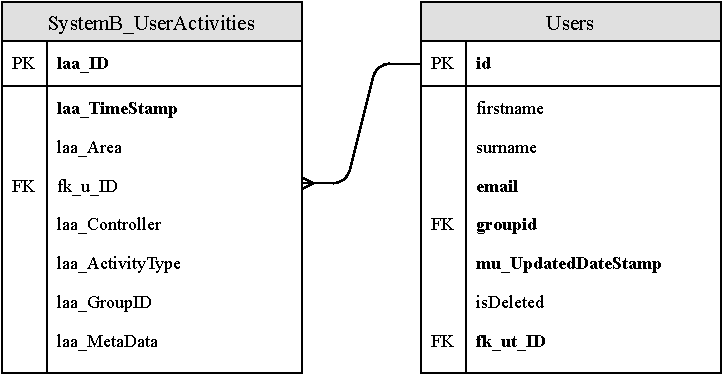
\includegraphics[width=0.9\textwidth]{Images/Chapter2/SystemB_ERD_Basic/SystemB_ERD_Basic.pdf}
	\caption[System B user activity ERD]
	{\textit{System B user activity ERD}}\label{fig:ch2_SystemB_Basic_ERD}
\end{figure}

\begin{figure}[!htb] % An h :here, t: top, b: bottom.
	\centering % cent the figure
	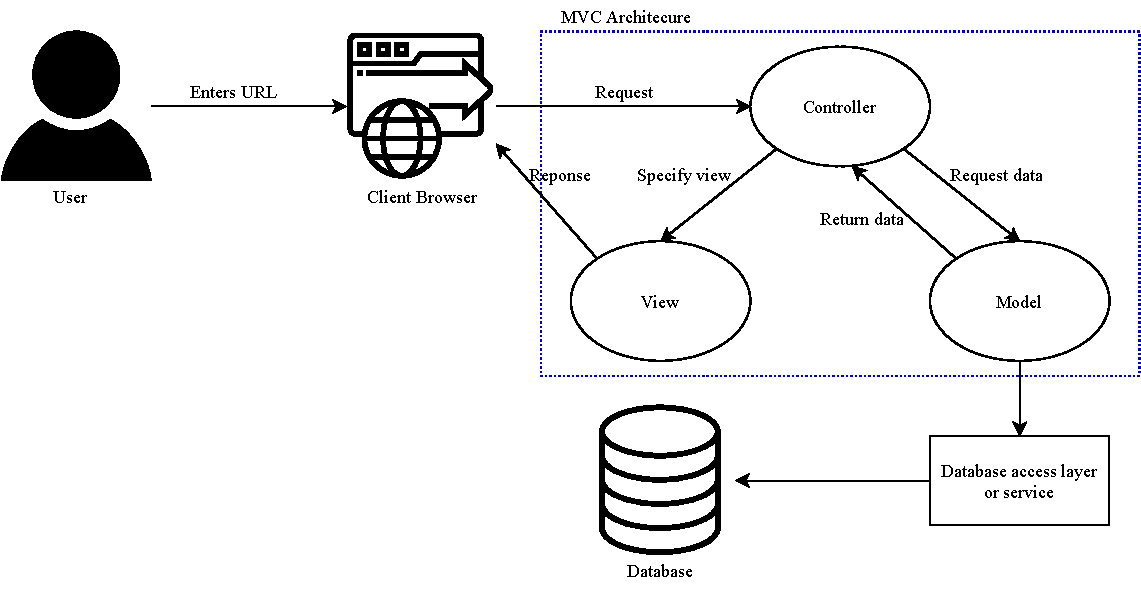
\includegraphics[width=0.95\textwidth]{Images/Chapter2/Flow_MVC_Architecture/Flow_MVC_Architecture.pdf}
	\caption[Request flow in MVC architecture]
	{\textit{Request flow in MVC architecture \cite{Gu2010}}}\label{fig:ch2_Flow_MVC_Architecture}
\end{figure}

\clearpage

\subsection{System A logging mechanism design}

In \Cref{fig:ch2_SystemA_Arch_Design} is the design for the System A's logging mechanism that consist of two different operations two log the event data that is generated from the user. These two main operations are used based on where the event is generated from either the PHP or MVC software components. The logging mechanism consist of two main functional requirements (\textbf{F/R}) that two main operations will use.

\begin{figure}[!htb] % An h :here, t: top, b: bottom.
	\centering % cent the figure
	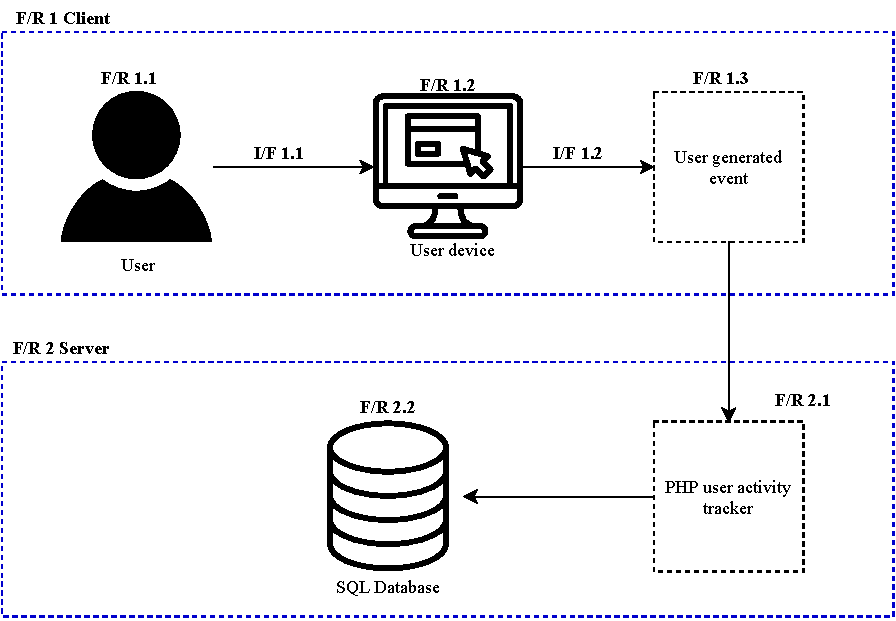
\includegraphics[width=0.99\textwidth]{Images/Chapter2/SystemA_Architecture_Diagram/SystemA_Architecture_Diagram.pdf}
	\caption[System A logging mechanism architecture design]
	{\textit{System A logging mechanism architecture design}}\label{fig:ch2_SystemA_Arch_Design}
\end{figure}

\section{System utilisation analysis}

\section{Integration}
In this section the integration of the utilisation analysis and logging mechanism will be discussed.

\section{Conclusion}
Conclude the chapter about the development of the logging mechanism and utilisation analysis.